  \subsection{Liczba kolorująca}
    Czy jesteśmy w stanie ograniczyć liczbę kolorującą przez funkcję od liczby klikowej w grafie przecięć prostokątów na płaszczyźnie?
    \begin{theorem}
        Nie.
    \end{theorem}
    \begin{proof}
        Możemy stworzyć klikę $K_{n,n}$ w tej klasie grafów. No i w sumie tyle. 
        \begin{figure}[H]
            \centering
            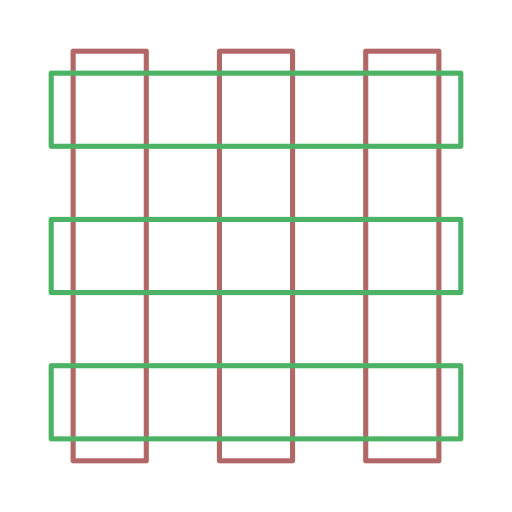
\includegraphics[scale=0.35]{images/objects_on_plane/k_3_3_of_rectangles.png}
            \caption{$K_{3,3}$ jako przecięcia prostokątów}
        \end{figure}
    \end{proof}
    \subsection{Liczba chromatyczna}
    
    Nie potrafimy ograniczyć liczby kolorującej to może chociaż chromatyczną umiemy? Okazuje się, że tak.
    \begin{theorem}
      Liczba chromatyczna w grafach przecięć prostokątów na płaszczyźnie ograniczona jest przez $\omega \cdot (8\omega - 7)$.
    \end{theorem}
    \begin{proof}
        Kolorujemy prostokąty na płaszczyźnie w dość zabawny sposób, bo każdy kolor będzie składał się z pary liczb. 
        Pierwsza współrzędna będzie przyjmowała wartości od $1$ do $\omega$, natomiast druga od $1$ do $8\omega - 7$.
        Intuicyjnie będzie odpowiadało to podzieleniu prostokątów na $\omega$ warstw, z których każdą z osobna będziemy umieli pokolorować na $8\omega - 7$ kolorów.
        
        Zacznijmy od pierwszej współrzędnej. 
        Powiemy, że dwa prostokąty \textbf{krzyżują się} jeśli przecinają się, ale wnętrze (bez brzegu) jednego nie zawiera wierzchołków drugiego.
        Jeżeli skierujemy relację krzyżowania w ten sposób, że
        $u \leq v$ gdy $u$ jest węższy niż $v$ to okazuje się, że dostaniemy częściowy porządek. 
        Możemy zauważyć, że łańcuch w tym porządku to ciąg coraz węższych i dłuższych prostokątów o wspólnym ,,środku'', więc tworzą one klikę o maksymalnym rozmiarze $\omega$.
        
       \begin{figure}[H]
            \centering
            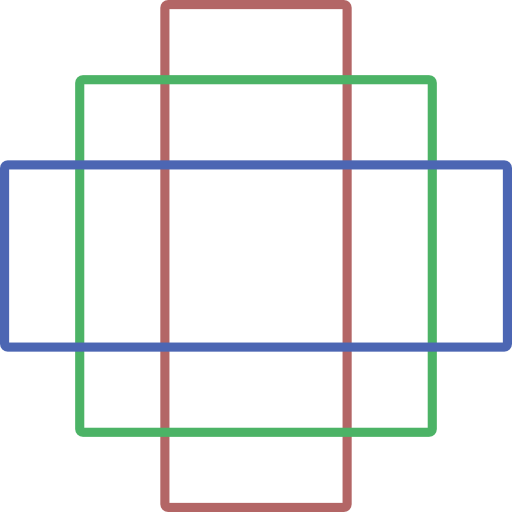
\includegraphics[scale=0.75]{images/objects_on_plane/rectangle_clique.png}
            \caption{,,Krzyżujące się'' prostokąty tworzące klikę; każdy prostokąt dostaje inny kolor na pierwszej współrzędnej}
        \end{figure}
        
        
        Skoro rozmiar najdłuższego łańcucha to $\omega$ to możemy skorzystać z twierdzenia dualnego do Dilwortha i podzielić prostokąty na $\omega$ antyłańcuchów $A_1, ..., A_\omega$,
        które intuicyjnie będą odpowiadały grupom prostokątów, które się nie krzyżują parami.
        Następnie na pierwszej współrzędnej każdy prostokąt dostaje numer antyłańcucha do którego trafił.
        
        Okazuje się, że dla prostokątów mających ten sam pierwszy kolor (a więc takich które się nie krzyżują) jesteśmy już w stanie ograniczyć liczbę kolorującą, a więc i liczbę chromatyczną. Robimy to w dosyć sprytny sposób.  Mianowicie zauważamy, że skoro prostokąty się nie krzyżują, gdy przecinają się one to musi być tak że jakiś wierzchołek jednego jest w drugim (lub vice versa).

        Co robimy z tym fascynującym faktem? Otóż majstrujemy sobie graf \textbf{skierowany} na prostokątach w taki sposób, 
        że krawędź z prostokąta $u$ do prostokąta $v$ mamy, gdy $u$ ma wierzchołek wewnątrz $v$.
        \begin{figure}[H]
            \centering
            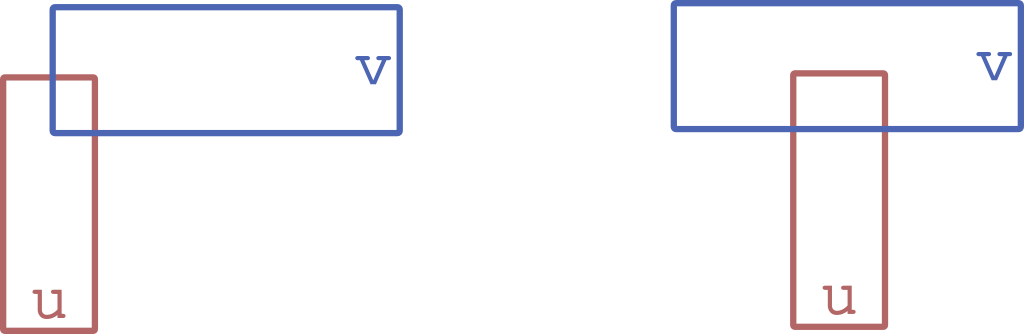
\includegraphics[scale=0.75]{images/objects_on_plane/rectangle_edges.png}

            \caption{po lewej mamy krawędzie $(u, v)$ oraz $(v, u)$, po prawej tylko $(u, v)$}
        \end{figure}
        
        Podobnie jak przy grafach przecięć kwadratów, zauważamy że z jednego prostokąta może wychodzić maksymalnie $4\omega - 4$ krawędzi (bo każdy wierzchołek może się zawierać w co najwyżej $\omega - 1$ prostokątów).
        W takim razie oszacowanie górne na liczbę krawędzi w grafie wynosi $|E| \leq |V| \cdot (4\omega - 4)$. Jednocześnie wiemy, że \begin{equation*}
          \sum_{v \in V} deg(v) = 2 \cdot |E|
      \end{equation*}
      Skąd
      \begin{equation*}
          \sum_{v \in V} deg(v) = 2 \cdot |E| \leq |V| \cdot (8 \omega - 8)
      \end{equation*}
      \begin{equation*}
          \frac{\sum_{v \in V} deg(v)}{|V|} \leq 8 \omega - 8
      \end{equation*}
      Należy zauważyć, że po lewej stronie mam średnią arytmetyczną stopni wszystkich wierzchołków w tym grafie. Ponieważ jest ona mniejsza lub równa $8 \omega - 8$, to wiem że istnieje na pewno wierzchołek który ma stopień mniejszy bądź równy $8\omega - 8$ (tak działa średnia arytmetyczna). To oczywiście tłumaczy się na to, że istnieje prostokąt o maksymalnym stopniu $8\omega - 8$ w grafie przecięć prostokątów. No a skoro tak, to prostokąt taki mogę sobie zawsze ,,wrzucić'' zawsze na koniec permutacji do liczby kolorującej, ,,odgryźć'' go od grafu i znowu wrzucić prostokąt o takim maksymalnym stopniu i tak dalej. Tym samym osiągnęliśmy ograniczenie na liczbę kolorującą w postaci $col(G) \leq 8\omega - 7$ (czyli również ograniczyliśmy liczbę możliwych kolorów ,,na drugiej współrzędnej'' w ten sposób). 
      
      Podsumowując: skoro na pierwszej współrzędnej mamy $\omega$ możliwych wartości, a na drugiej $8\omega - 7$ to razem używamy $\omega \cdot (8\omega - 7)$ kolorów.
      
    \end{proof}